  %%%%%%%%%%%%%%%%%%%%%%%%%%%%%%%%%%%%%%%%%%%%%%%%%%%%%%%%%%%%%%%%%%%%%%%%%%%%% 
%
% This is a LaTeX file for an A0 poster.
% 
% template poster taken from https://canizo.org/latex_poster
%
%%%%%%%%%%%%%%%%%%%%%%%%%%%%%%%%%%%%%%%%%%%%%%%%%%%%%%%%%%%%%%%%%%%%%%%%%%%%% 

%%%%%%%%%%%%%%%%%%%%%%%%%%%%%%%%%%%%%%%%%%%%%%%%%%%%%%%%%%%%%%%%%%%%%%%%%%%%% 
%%%%%%%%%%%%%%%%%%%%%%%%%%%%%%%%%%%%%%%%%%%%%%%%%%%%%%%%%%%%%%%%%%%%%%%%%%%%%
%
% Towards a standardized workflow for mass spectrometry based single-cell 
% proteomics
%
% Poster for the Applied Bioinformatics for Life Science, February 2020.
%
%%%%%%%%%%%%%%%%%%%%%%%%%%%%%%%%%%%%%%%%%%%%%%%%%%%%%%%%%%%%%%%%%%%%%%%%%%%%%
%%%%%%%%%%%%%%%%%%%%%%%%%%%%%%%%%%%%%%%%%%%%%%%%%%%%%%%%%%%%%%%%%%%%%%%%%%%%%

\documentclass{article}
% To modify the size of the page:
\usepackage[dvips,a3paper,portrait,centering,margin=0.5cm]{geometry}
% To create multiple columns
\usepackage{multicol}

\usepackage[utf8]{inputenc}
% To align images
\usepackage[export]{adjustbox}
% Use captions in minipages
\usepackage{caption}
% Math font
\usepackage{amsmath, amsthm, amsfonts}
% Include figure files.
\usepackage{graphicx}

% Coding fonts
% ------------
% For including R chunks 
\usepackage{listings} 
\lstset{
  language=R,
  basicstyle=\small\ttfamily\color{vdgray},       % the size of the fonts that are used for the code
  % sensitive=false,
  numbers=left,                   % where to put the line-numbers
  numberstyle=\tiny\color{gray},  % the style that is used for the line-numbers
  stepnumber=1,                   % the step between two line-numbers.
  numbersep=0.1cm,                % how far the line-numbers are from the code
  backgroundcolor=\color{lgray},  % choose the background color. You must add \usepackage{color}
  deletekeywords={stat},
  keywordstyle=\color{blue},      % keyword style
  stringstyle=\color{green},      % string literal style
  xleftmargin=0.5cm,
}
% Create command for highlighting inline code or variables
\newcommand{\hcode}[2][lgray]{{\ttfamily\color{vdgray}\colorbox{#1}{#2}}}

% Colors
% ------
\usepackage{color}
\usepackage[dvipsnames]{xcolor}
% Color panel used throughout the poster
\definecolor{lgray}{rgb}{0.9179688,0.9179688,0.9179688} % #ebebeb
\definecolor{dgray}{rgb}{0.796875,0.796875,0.796875} % #cccccc
\definecolor{vdgray}{rgb}{0.3984375,0.3984375,0.3984375} % #666666
\definecolor{coral}{rgb}{0.9960938,0.4960938,0.3125000} % #ff7f50
\definecolor{blue}{rgb}{0.4218750,0.6484375,0.8007812} % #6ca6cd
\definecolor{green}{rgb}{0.6992188,0.7265625,0.5078125} % #b3ba82
\definecolor{yellow}{rgb}{0.9570312,0.8671875,0.6992188} % #f5deb3

% Adjust space between reference items
% ------------------------------------
\let\OLDthebibliography\thebibliography
\renewcommand\thebibliography[1]{
  \OLDthebibliography{#1}
  \setlength{\parskip}{0pt}
  \setlength{\itemsep}{0pt plus 0.3ex}
}
  
\pagestyle{empty}

\def\to{\rightarrow}


% ===========================================================================

\title{}
\author{}
\date{}

\begin{document}

% ---------------------------------------------------------------------------
% Data Visualization 
\noindent
\begin{minipage}[t]{\linewidth}
  \vspace{0.5cm}
  \section*{\huge Data Visualization}
  \large
  \hcode{scpdata} also offers an ideal environment for benchmarking. It will contain a wide variety of MS-SCP data sets from \textbf{well-defined synthetic standards} to \textbf{real biological samples}. Different methods can be compared using \textbf{objective benchmarking metrics} or \textbf{visualization} with dimension reduction (Figure \ref{fig:pca}).
  \begin{center}
    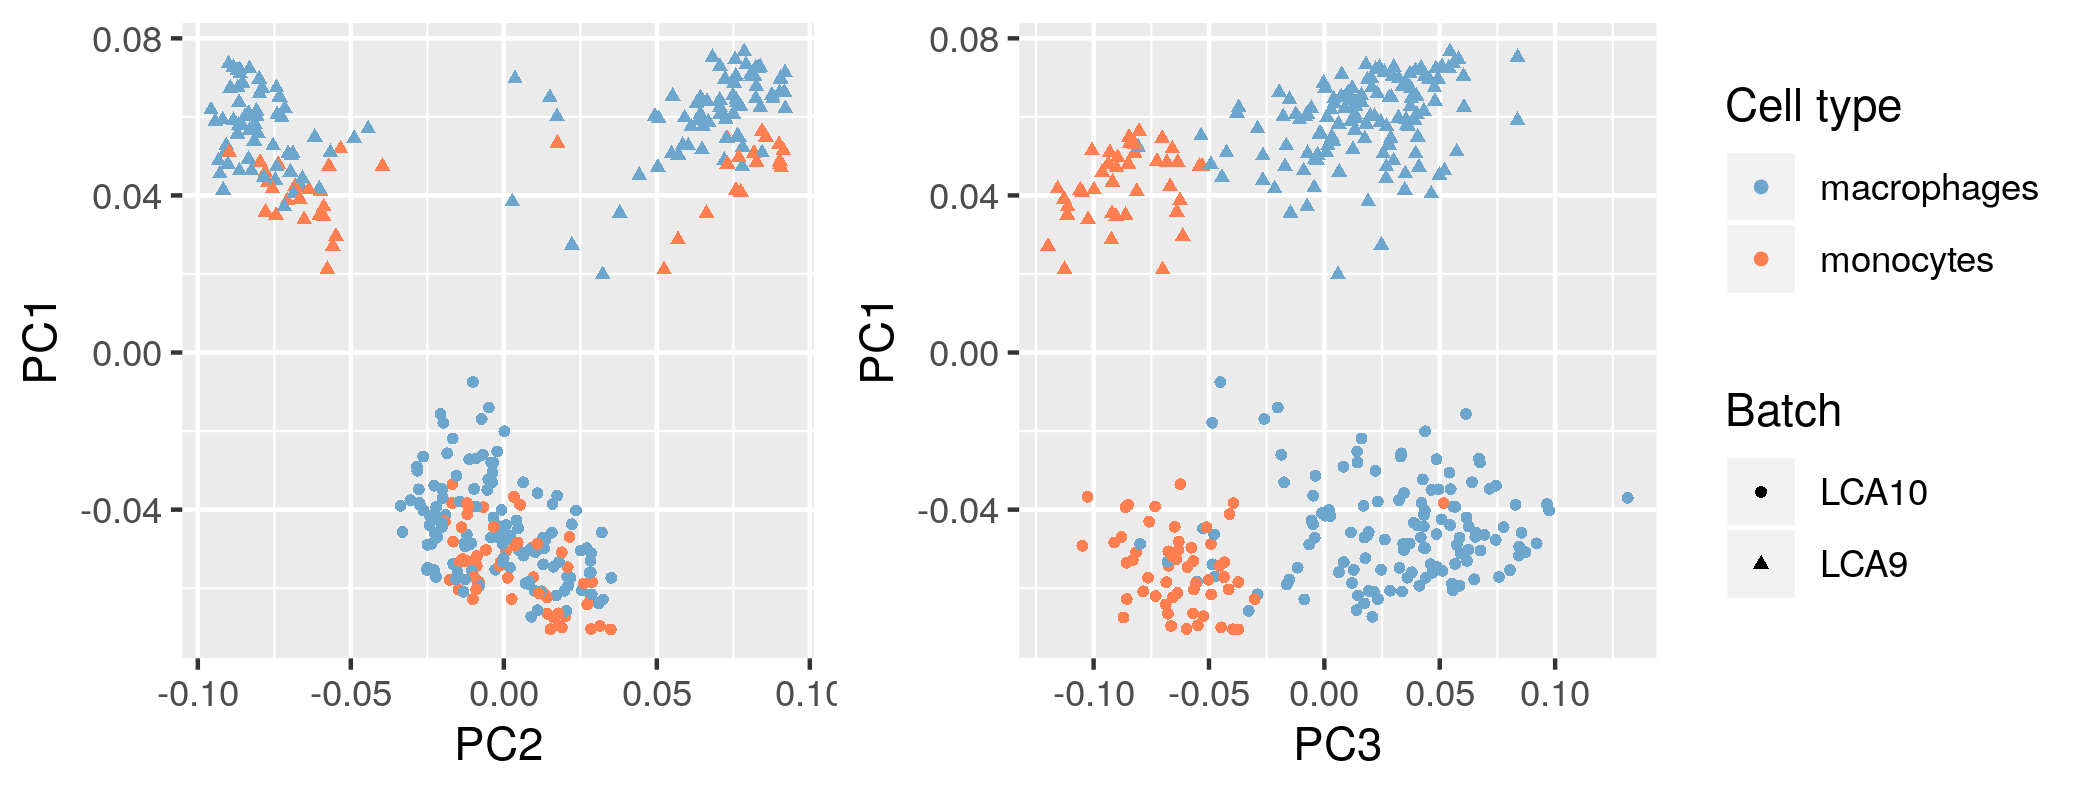
\includegraphics[width=\textwidth]{figs/PCA.png}
  \end{center}
  \captionof{figure}{\textbf{PCA plot of peptide expression data.} \small Macrophages and monocytes are well separated in the third principal component. However, the first and second components are driven by batch effects. LCA10 and LCA9 are two chromatographic batches. The PCA was performed using the NIPALS algorithm.}
  \label{fig:pca}

\end{minipage}

% ---------------------------------------------------------------------------
% Problems to tackle
\noindent
\begin{minipage}[t]{\linewidth}
  \vspace{0.35cm}
  \section*{\huge Problems to tackle}
  \vspace{0.15cm}
\end{minipage}
  
% Batch effect
\noindent
\begin{minipage}[h]{0.35\linewidth}
  \subsection*{Batch effects}
  \large
  Batch effects are inherent to MS-SCP data since many samples/cells have to be distributed across \textbf{different MS runs}. This leads to major biases in the data (Figure \ref{fig:pca}).
% Missingness
  \subsection*{Missingness}
  \captionof{figure}{\textbf{Distribution of missing data in monocytes against macrophages.} \small The average missingness is $\pm$ 75 \%. Color indicates the log2 fold change of \textbf{\color{coral}macrophages} over \textbf{\color{green}monocytes} relative expression. Data from \cite{Specht2019-jm}.}
  \label{fig:missing}
  \begin{center}
  \end{center}
\end{minipage}
\hspace{0.4cm}
% Missingness figure
\begin{minipage}[h]{0.6\linewidth}
  \begin{center}
  
\includegraphics[width=0.5\linewidth, trim={10cm 3cm 7cm 0},clip]{figs/missing-leg.png}
  \end{center}
  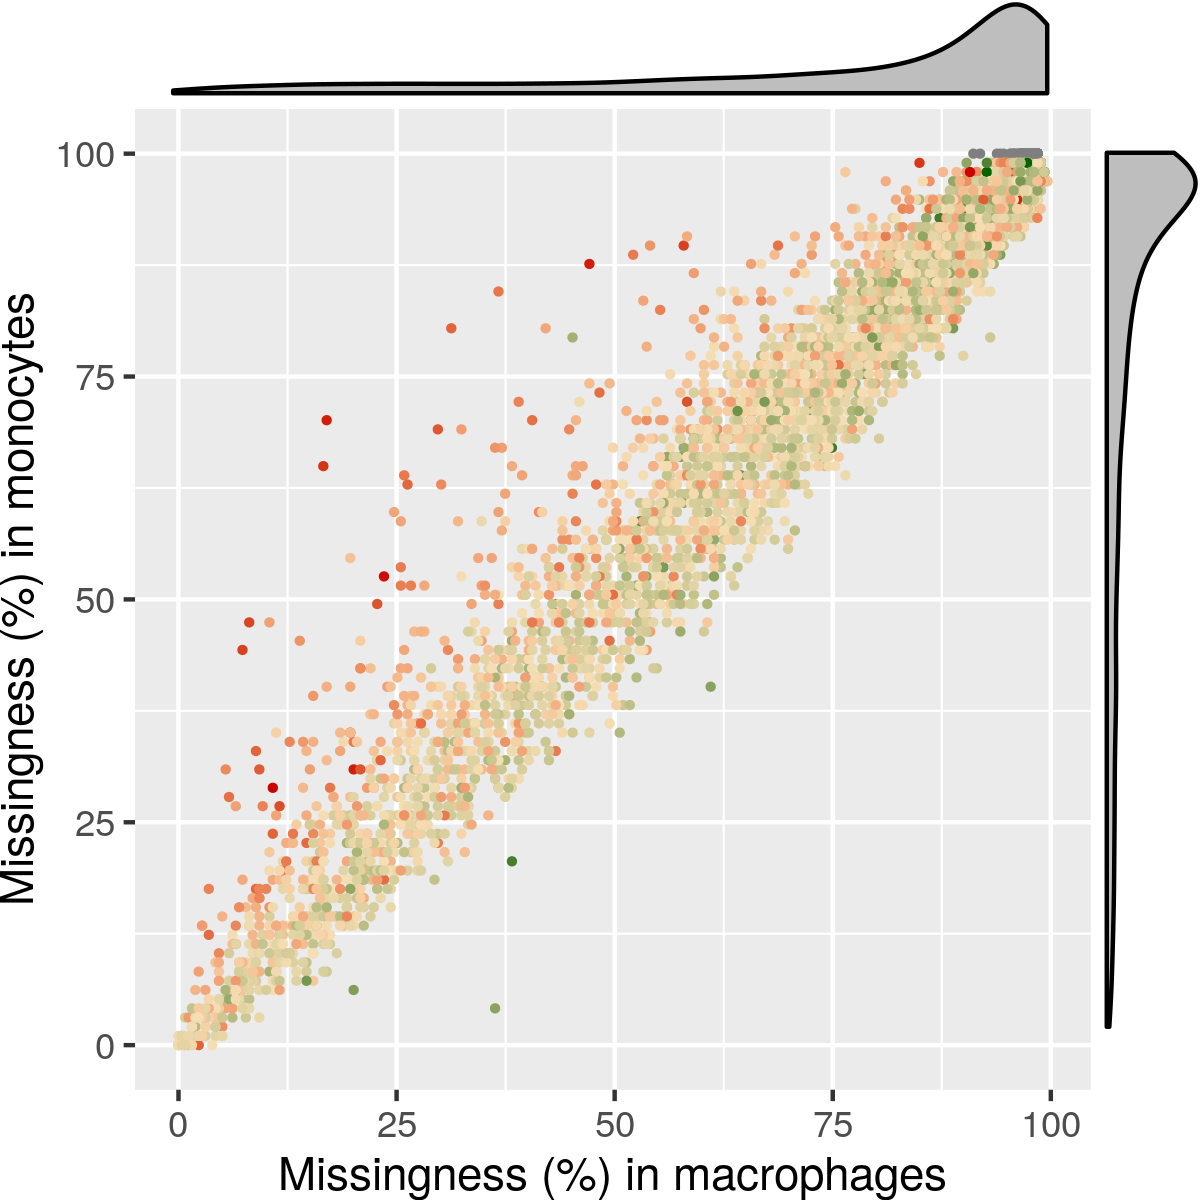
\includegraphics[width=\linewidth, trim={0 2cm 0 2cm}]{figs/missing.png}
\end{minipage}

% Curse of dimensionality
\noindent
\begin{minipage}[h]{\linewidth}
  \subsection*{Curse of dimensionality}
  \large
  Although current acquisition pipelines produce data sets of \textbf{thousands of peptides x hundreds of cells}, it is expected that new technological advances might raise the dimensionality 100 fold \cite{Specht2019-jm}. This is a challenge for the \textbf{statistical analyses} and for the \textbf{software optimization}. Possible solutions should be inspired from current achievements in single cell transcriptomics. 
\end{minipage}

% ---------------------------------------------------------------------------
% Additional notes
\vspace{0.5cm}
\noindent
This work is funded by an Aspirant FRS-FNRS fellowship awarded to Christophe Vanderaa. The poster is available at {\color{blue}{https://github.com/cvanderaa/EuroBioc2019-Poster}}.



% ---------------------------------------------------------------------------
% References
\scriptsize
\bibliography{ref.bib} 
\bibliographystyle{ieeetr}

% ---------------------------------------------------------------------------
% End of poster
\end{multicols}
\end{document}